\documentclass[../main.tex]{subfiles}
\begin{document}
\paragraph{New probabilistic upper bounds}\label{par:new_bounds}
We formulate the polynomial least-squares problem derived above in a statistical sense so that we can perform rigorous error analysis.
To start, we make explicit the dependence of the dependent variables $y_{j}$ on some r.v.s which we assume to be standard distributed.
The problem is thus formulated as follows: given a set of $n$ nodes $\{x_{1},\dots,x_{n}\}$ we record $n$ observations of the form $y_{j} = f(x_{j}) + \xi_{j}$ where $f$ is prescribing the deterministic trend in the data and it is subject to random perturbations modelled as r.v.s $\xi_{j}\sim \mathcal{N}(0,\sigma^2)$.
The polynomial least-squares thus finds a set of $m<n$ coefficients $\{c_{1},\dots,c_{m}\}$ by solving the normal equations \eqref{eq2.5.2.3}.
Let us denote $\boldsymbol{A}^{+}=:\boldsymbol{H}\in \mathbb{R}^{m\times n}$, $\boldsymbol{b}=:\boldsymbol{y}\in \mathbb{R}^{n}$ and explicitly write the solution as $\boldsymbol{c} = \boldsymbol{Hy}\in \mathbb{R}^{m}$.
Since we made the dependence of the observations of the dependent variables $\boldsymbol{y}$ on the normally distributed r.v.s $\boldsymbol{\xi}=(\xi_{1},\dots,\xi_{n})$ then we conclude that the coefficients are themselves r.v.s through a linear function $\boldsymbol{c} = g(\boldsymbol{y}) = \boldsymbol{Hy}$.
Two questions arise: first is can we say something about the distribution of $\boldsymbol{c}$? And second is what are the errors associated to the solution $\boldsymbol{c}$?
Given this two-fold analytical aspects we refer to this sub-paragraph as the statistical error analysis of a polynomial least-squares problem.
Let us write the expression for the $j-$th coefficient as a solution of the least-squares problem
\begin{equation}\label{eq2.5.2.4}
        c_{j} = \sum_{k=1}^{n}H_{jk}y_{k} = \sum_{k=1}^{n}H_{jk}f(x_{k}) + \sum_{k=1}^{n}H_{jk}\xi_{k} = \overline{c_{j}} + \sum_{k=1}^{n}H_{jk}\xi_{k}\,.
\end{equation}
Notice that the deterministic quantity $\overline{c_{j}} := \sum_{k=1}^{n}H_{jk}f(x_{k})$ is nothing else then the solution of the least-squares problem \eqref{eq2.5.2.3} in the absence of noise (i.e. interpolating every observation $y_{j} = f(x_{j})$) exactly so that the residual is $r(\boldsymbol{c}) = 0$.
Furthermore $\overline{c_{j}}$ is the sample mean of the distribution of the $c_{j}$ r.v., hence the overbar notation we adopted.
It is reasonable to assume that $\mathbb{E}(c_{j})\to\overline{c_{j}}$ in some asymptotic sense; in fact we notice that by defining the quantity
\begin{equation}\label{eq2.5.2.5}
     \hat{c}_{j}:=c_{j} - \overline{c_{j}} = \sum_{k=1}^{n}H_{jk}\xi_{k}\,,
\end{equation}
and assuming that $H_{jk}=\frac{1}{n}$, $k=1,\dots,n$ then, by the Central Limit Theorem, we get
\begin{equation*}
        \sqrt{n}\hat{c}_{j}\xrightarrow{d}\mathcal{N}(0,\sigma^{2})\,.
\end{equation*}
Since in general $H_{jk}\neq \frac{1}{n}$, we need to study the convergence of $\hat{c}_{j}$ with a different approach.
Let us start by taking the absolute value ($L_{1}-$norm) of \eqref{eq2.5.2.5}
\begin{equation}\label{eq2.5.2.6}
        |\hat{c}_{j}| = |c_{j} - \overline{c_{j}}| = \bigg|\sum_{k=1}^{n}H_{jk}\xi_{k}\bigg|\,.
\end{equation}
A naive upper bound is derived for \eqref{eq2.5.2.6} by applying the triangle inequality and realising that since $\xi_{k}\sim \mathcal{N}(0,\sigma^{2})$ then $P(|\xi_{k}|\leq3\sigma)=1$ and hence
\begin{equation}\label{eq2.5.2.7}
        |\hat{c}_{j}| = \Bigg|\sum_{k=1}^{n}H_{jk}\xi_{k}\Bigg|\leq\sum_{k=1}^{n}|H_{jk}||\xi_{k}|\stackrel{a.a.}{\leq}3\sigma\sum_{k=1}^{n}|H_{jk}|\,.
\end{equation}
From \eqref{eq2.5.2.7} we can deduce the upper estimate
\begin{equation}\label{eq2.5.2.8}
     |\hat{c}_{j}|\leq3\sigma ||H||_{\infty} \leq3\sigma n ||H||_{\text{max}}\,,
\end{equation}
where in we used the matrix norms $||H||_{\infty} = \max_{j=1,\dots,m}\sum_{k=1}^{n}|H_{jk}|$ and $||H||_{\text{max}} = \max_{j,k}|H_{jk}| $. 
Notice that the less tight upper estimates in \eqref{eq2.5.2.8} provides an explicit dependence on $n$ which is linear, meaning that it will monotonically increase as the number of observations increases.
This is clearly not ideal however, as evidenced by Figure \ref{fig2.5.2.2}, we know that such increase is bounded from above.
Nevertheless, we wish to derive a better upper estimate that decreses monotonically with $n$ and to do that we must somehow exploit the structure of the pseudoinverse $\boldsymbol{H}$.
To do this let us observe first that $|\hat{c}_{j}| = |\sum_{k=1}^{n}H_{jk}\xi_{k}|$ is the inner product between the $j-$th row vector $\boldsymbol{H}_{j}\in \mathbb{R}^{n}$ and the vector of i.i.d. normally-distributed r.v.s $\boldsymbol{\xi}$.
Therefore using Cauchy-Schwarz inequality we can write
\begin{equation}\label{eq2.5.2.9}
        |\hat{c}_{j}| = \Bigg|\sum_{k=1}^{n}H_{jk}\xi_{k}\Bigg| = |\boldsymbol{H}_{j}\cdot \boldsymbol{\xi}|\leq||\boldsymbol{H}_{j}||_{2}||\boldsymbol{\xi}||_{2}\leq3\sigma\sqrt{n}||\boldsymbol{H}_{j}||_{2}\,,
\end{equation}
where $||\cdot||_{2}$ denotes the $L_{2}$ vector norm.
For any rectangular matrix $\boldsymbol{M}\in \mathbb{R}^{n\times m}$ with $m<n$ this norm induces the so-called \textit{spectral norm} which corresponds exactly with the square root of the largest eigenvalue of $\boldsymbol{M}^{T}\boldsymbol{M}$.
Now let $\boldsymbol{M}=\boldsymbol{U}\boldsymbol{\Sigma}\boldsymbol{V}^{T}$ be the singular value decomposition of $\boldsymbol{M}$, where $\mathbb{R}^{n\times m}\ni\boldsymbol{\Sigma} = \text{diag}(\sigma_{1},\dots,\sigma_{m})$ then the spectral norm coincides with its largest singular value i.e. $||\boldsymbol{M}||_{2}=\sqrt{\max_{\lambda}(\boldsymbol{M}^{T}\boldsymbol{M})} = \sigma_{1}$.
Finally denoting $\boldsymbol{M}^{+}$ as the pseudoinverse of $\boldsymbol{M}$ then its singular value decomposition is well known $\boldsymbol{M}^{+} = \boldsymbol{V}\boldsymbol{\Sigma}^{-1}\boldsymbol{U}^{T}$ where $\boldsymbol{\Sigma} = \text{diag}(\sigma_{m}^{-1},\dots,\sigma_{1}^{-1})$ so that $||\boldsymbol{M}^{+}||=\frac{1}{\sigma_{m}}$, i.e. the spectral norm of the pseudoinverse of $\boldsymbol{M}$ is the reciprocal of the smallest singular value of $\boldsymbol{M}$.
\begin{figure}[H]
    \centering 
    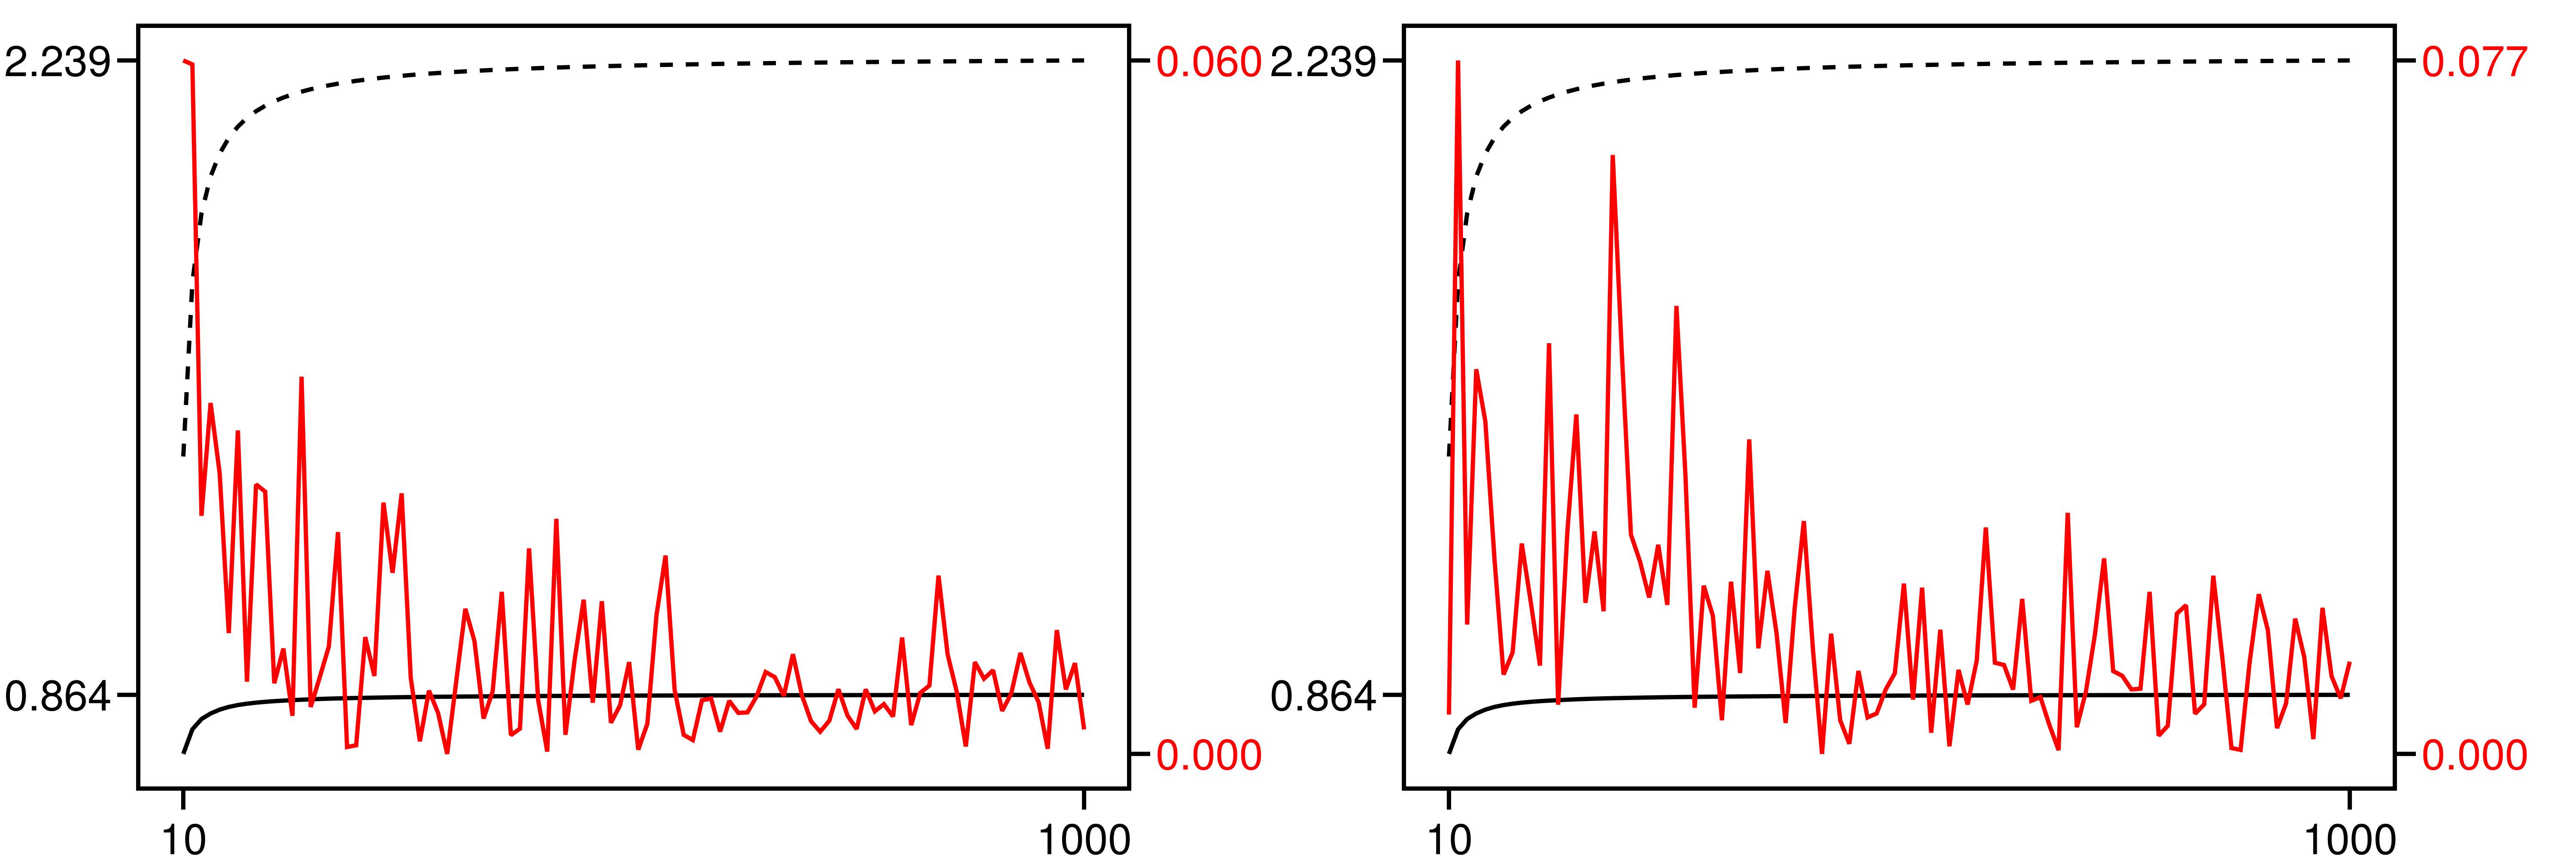
\includegraphics[keepaspectratio, width=\textwidth]{../figures/fig2.5.2.2.png}
    \caption{Comparison between the convergence with $n$ of the exact numerical errors (red solid line) and the upper estimates $3\sigma||H||_{\infty}$ (black solid lines) and $3\sigma n ||H||_{\text{max}}$ (black dashed lines) in \eqref{eq2.5.2.8} for a quadratic ($m=3$) least-square regression observations with standard deviation $\sigma=0.1$. 
    Linear coefficient $c_{1}$ on the left and the quadratic coefficient $c_{2}$ on the right.}
    \label{fig2.5.2.2}
\end{figure}
Equipped with these facts we can find an upper estimate from \eqref{eq2.5.2.9}
\begin{equation}\label{eq2.5.2.10}
        |\hat{c}_{j}|\leq3\sigma\sqrt{n}||\boldsymbol{H}_{j}||_{2}\leq3\sigma\sqrt{n}||\boldsymbol{H}||_{2} = \frac{3\sigma\sqrt{n}}{\sigma_{m}}\,,
\end{equation}
where $\sigma_{m}$ denotes the smallest singular value of $\boldsymbol{A}$.
We can now introduce the Frobenius matrix norm $||\boldsymbol{M}||_{F}=\sqrt{\sum_{j=1}^{m}\sigma_{j}^{2}}$ and state without proof that $||\boldsymbol{M}||_{2}\leq||\boldsymbol{M}||_{F}$.
It follows trivially that $||\boldsymbol{M}||_{F}\leq\sigma_{1}\sqrt{m}$ and thus $||\boldsymbol{M}^{+}||_{F}\leq \frac{\sqrt{m}}{\sigma_{m}}$ which we use in \eqref{eq2.5.2.10} to get
\begin{equation}\label{eq2.5.2.11}
     |\hat{c}_{j}|\leq\frac{3\sigma\sqrt{n}}{\sigma_{m}}\leq\frac{3\sigma\sqrt{nm}}{\sigma_{m}}\,.
\end{equation}
The dependence on $n$ in \eqref{eq2.5.2.11} is still monotonically increasing albeit at a slower rate and we also made it explicit the dependence on the number of polynomial coefficients $m$.
\begin{figure}[H]
    \centering 
    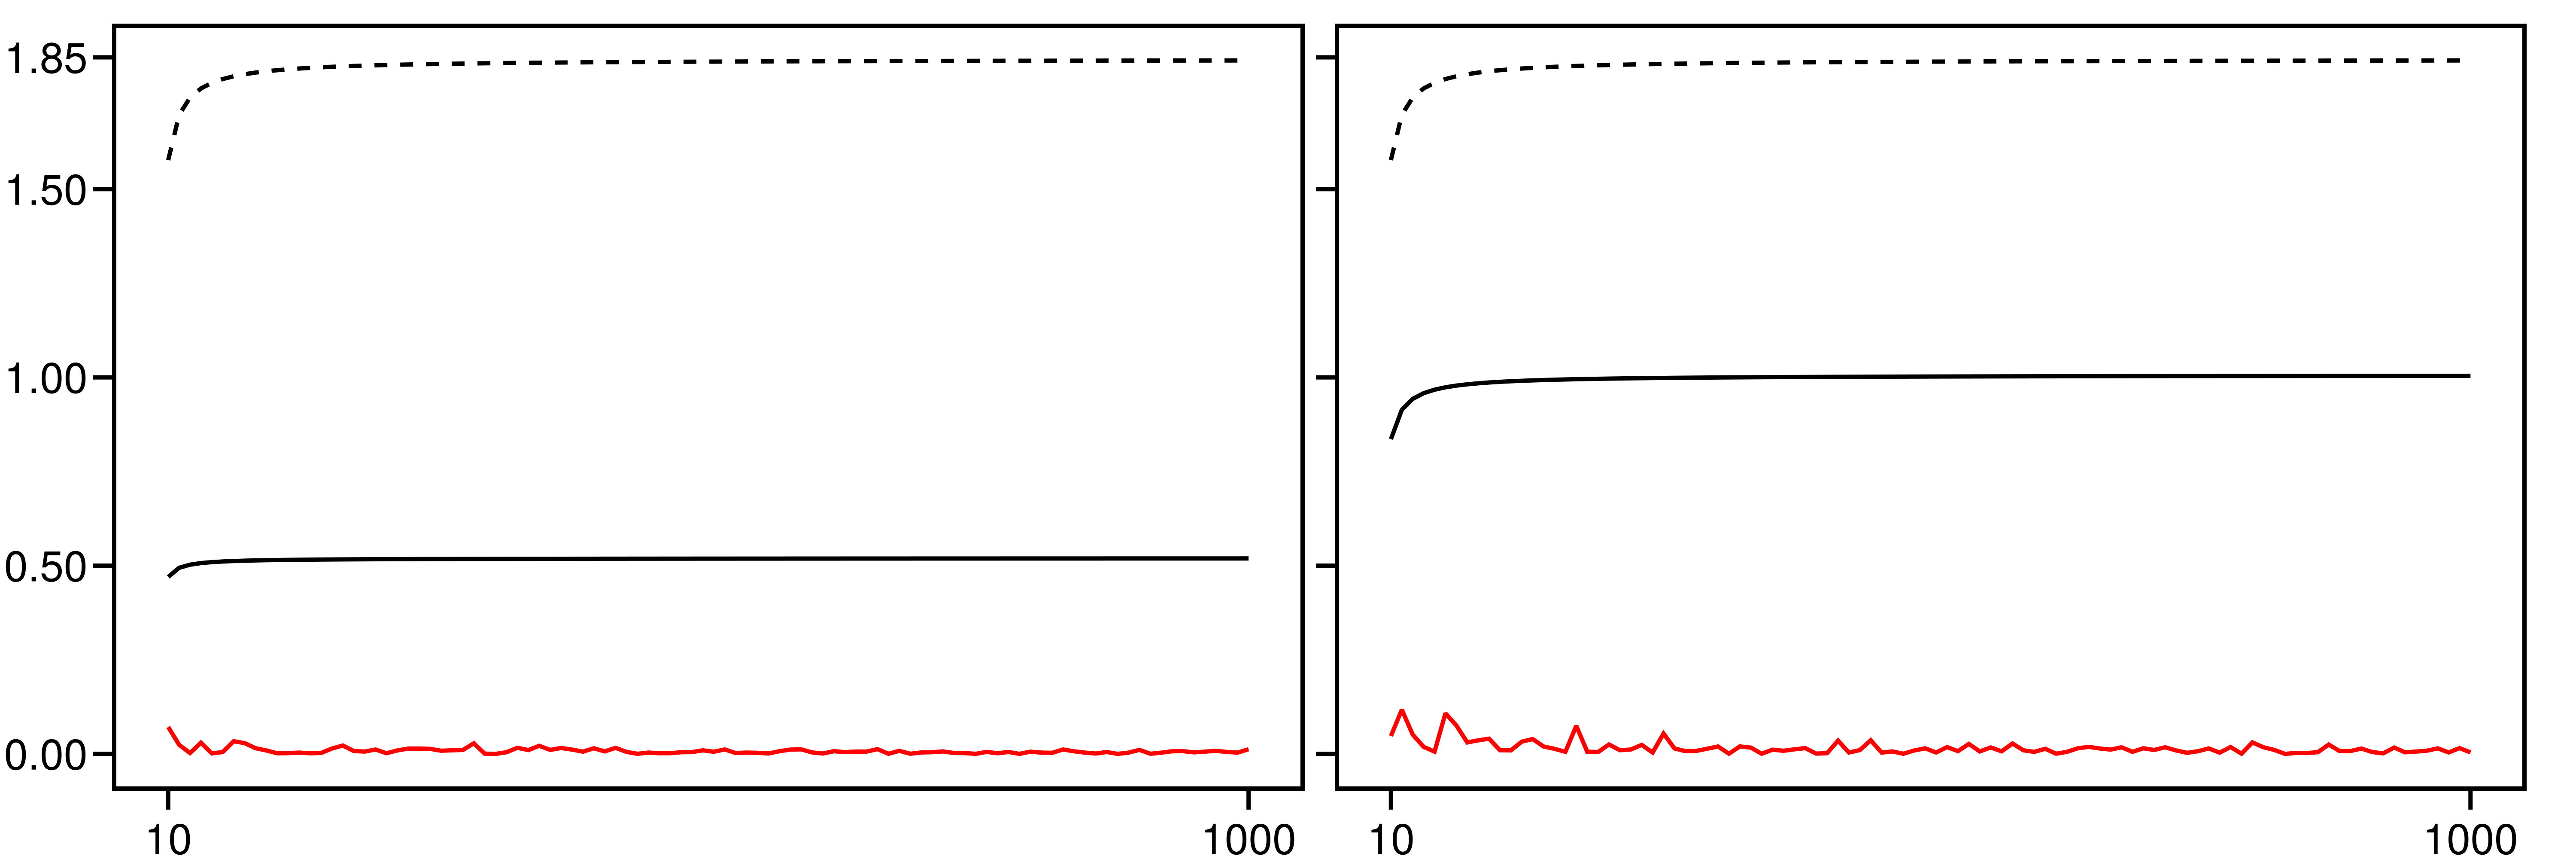
\includegraphics[keepaspectratio, width=\textwidth]{../figures/fig2.5.2.3.png}
    \caption{Comparison between the convergence with $n$ of the exact numerical errors (red solid lines) and the upper estimates \eqref{eq2.5.2.9} (black solid lines) and \eqref{eq2.5.2.11} (black dash lines) for the same fit of Figure \ref{fig2.5.2.2}.}
    \label{fig2.5.2.3}
\end{figure}
A new approach is required to derive the desired asymptotic decay of the error with the number of samples $n$.
So far in fact we treated the RHS of the estimate as a statistical quantity due to the presence of the normally-distributed r.v.s $\xi_{j}$ but have left the error itself on the LHS $|\hat{c}_{j}| = |c_{j}-\overline{c_{j}}|$ as a deterministic quantity.
Therefore let us modify \eqref{eq2.5.2.6} by taking its expected value
\begin{equation}\label{eq2.5.2.12}
        \mathbb{E}(\hat{c}_{j}) = \mathbb{E}\Bigg(\Bigg|\sum_{k=1}^{n}H_{jk}\xi_{k}\Bigg|\Bigg)\,.
\end{equation}
In general, if $x$ is a r.v. and $g$ a reasonable function of $x$ then it holds that $\mathbb{E}(g(x))\neq g(\mathbb{E}(x))$.
However, as we mentioned at the beginning of the sub-paragraph, if $g$ is linear, then, by linearity of the expectation operator, the inequality becomes an identity $\mathbb{E}(g(x)) = g(\mathbb{E}(x))$.
In addition let $\{x_{1},\dots,x_{n}\}$ be i.i.d. with $x_{j}\sim \mathcal{N}(0,\sigma^{2})$, then it holds 
\begin{equation}\label{eq2.5.2.13}
        y = g(\{x_{1},\dots,x_{n}\}) = \sum_{j=1}^{n}\alpha_{j}x_{j}\sim \mathcal{N}(0,\sigma^{2}\sum_{j=1}^{n}\alpha_{j}^{2}=:\overline{\sigma^{2}})\,.
\end{equation}
Being $y\sim \mathcal{N}(0,\overline{\sigma^{2}})$ we know that $|y|$ has a folded normal distribution whose expectation value is
\begin{equation*}
        \mathbb{E}(|y|)=\sqrt{\frac{2}{\pi}}\overline{\sigma}\,,
\end{equation*}
which by \eqref{eq2.5.2.13} it becomes
\begin{equation}\label{eq2.5.2.14}
        \mathbb{E}\Bigg(\Bigg|\sum_{j=1}^{n}\alpha_{j}x_{j}\Bigg|\Bigg)=\sigma\sqrt{\frac{2}{\pi}\sum_{j=1}^{n}\alpha_{j}^{2}}\,.
\end{equation}
We can now put \eqref{eq2.5.2.12} into \eqref{eq2.5.2.14} to get
\begin{equation*}
        \mathbb{E}(|\hat{c}_{j}|) = \sigma\sqrt{\frac{2}{\pi}\sum_{k=1}^{n}H_{jk}^{2}}\leq\sigma\sqrt{\frac{2}{\pi}}||\boldsymbol{H}||_{2}=\sigma\sqrt{\frac{2}{\pi}\max_{\lambda}(\boldsymbol{H}^{T}\boldsymbol{H})}=\sigma\sqrt{\frac{2}{\pi}\max_{\lambda}(\boldsymbol{H}\boldsymbol{H}^{T})}\,,
\end{equation*}
which for convenience we square to get
\begin{equation}\label{eq2.5.2.15}
        \mathbb{E}^{2}(|\hat{c_{j}}|)\leq\frac{2\sigma^{2}}{\pi}\lambda_{\text{max}}(\boldsymbol{H}\boldsymbol{H}^{T})\,,
\end{equation}
where we adopted the notation $\max_{\lambda}(\boldsymbol{H}\boldsymbol{H}^{T})=:\lambda_{\text{max}}(\boldsymbol{H}\boldsymbol{H}^T)$.
Notice that since $\boldsymbol{H}=\boldsymbol{A}^{+}=(\boldsymbol{A}^{T}\boldsymbol{A})^{-1}\boldsymbol{A}^{T}$ then
\begin{equation*}
    \boldsymbol{H}\boldsymbol{H}^{T}=\bigg((\boldsymbol{A}^{T}\boldsymbol{A})^{-1}\boldsymbol{A}^{T}\bigg)\boldsymbol{A}(\boldsymbol{A}^{T}\boldsymbol{A})^{-1} = (\boldsymbol{A}^{T}\boldsymbol{A})^{-1}\,, 
\end{equation*}
which by eigendecomposition it thus gives us that
\begin{equation*}
     \sigma(\boldsymbol{H}\boldsymbol{H}^{T}) = \frac{1}{\sigma(\boldsymbol{A}^{T}\boldsymbol{A})}\,,
\end{equation*}
and in particular
\begin{equation}\label{eq2.5.2.16}
     \lambda_{\text{max}}(\boldsymbol{H}\boldsymbol{H}^{T}) = \frac{1}{\lambda_{\text{min}}(\boldsymbol{A}^{T}\boldsymbol{A})}\,.
\end{equation}
Putting \eqref{eq2.5.2.16} into \eqref{eq2.5.2.15} makes the estimate to depend explicitly on the model matrix $\boldsymbol{A}$
\begin{equation}\label{eq2.5.2.17}
      \mathbb{E}^{2}(|\hat{c_{j}}|)\leq\frac{2\sigma^{2}}{\pi\lambda_{\text{min}}(\boldsymbol{A}^{T}\boldsymbol{A})}\,,
\end{equation}
which now enables us to exploit the structure of $\boldsymbol{A}$ being a Vandermonde matrix.
To investigate that let us first write explicitly
\begin{equation*}
     \boldsymbol{A}^{T}\boldsymbol{A}=\begin{bmatrix}
             1 & 1 & 1 & \cdots & 1 & 1 \\
             x_{1} & x_{2} & x_{3} & \cdots & x_{n-1} & x_{n} \\
             x_{1}^{2} & x_{2}^{2} & x_{3}^{2} & \cdots & x_{n-1}^{2} & x_{n}^{2} \\
             \vdots & \vdots & \vdots & \cdots & \vdots & \vdots \\
             x_{1}^{m-1} & x_{2}^{m-1} & x_{3}^{m-1} & \cdots & x_{n-1}^{m-1} & x_{n}^{m-1} \\
     \end{bmatrix}\begin{bmatrix}
                        1 & x_{1} & x_{1}^{2} & \cdots  & x_{1}^{m-1} \\
                        1 & x_{2} & x_{2}^{2} & \cdots  & x_{2}^{m-1} \\
                        1 & x_{3} & x_{3}^{2} & \cdots  & x_{3}^{m-1} \\
                        \vdots &\vdots & \vdots & \cdots  & \vdots \\
                        1 & x_{n-1} & x_{n-1}^{2} & \cdots  & x_{n-1}^{m-1} \\
                        1 &x_{n} & x_{n}^{2} & \cdots  & x_{n}^{m-1}
                \end{bmatrix}
                =\Bigg[\sum_{\ell=1}^{n}x_{\ell}^{j+k-2}\Bigg]_{j,k=1}^{m}\,.
\end{equation*}
We are interested in the structure of $\boldsymbol{A}^{T}\boldsymbol{A}$ as a function of $n$ therefore we write
\begin{equation}\label{eq2.5.2.18}
     \boldsymbol{A}^{T}\boldsymbol{A} = n\Bigg[\frac{1}{n}\sum_{\ell=1}^{n}x_{\ell}^{j+k-2}\Bigg]_{j,k=1}^{m}\,.
\end{equation}
Putting \eqref{eq2.5.2.18} into \eqref{eq2.5.2.17} gives us
\begin{equation}\label{eq2.5.2.19}
     \mathbb{E}^{2}(|\hat{c_{j}}|)\leq\frac{2\sigma^{2}}{\pi n\lambda_{\text{min}}(\frac{1}{n}\boldsymbol{A}^{T}\boldsymbol{A})}\,,
\end{equation}
which is already promising since the dependence on $n$ is now monotonically decreasing compared to the previous estimates.
The next step is realising that each entry in \eqref{eq2.5.2.18} is nothing else but the normalised Riemann sum of the univariate monomial $f_{j,k} = x^{j+k-2}$.
\begin{interpretation*}{}
        Let $[a,b]\subset \mathbb{R}$ and $f:[a,b]\to \mathbb{R}$ bounded on $[a,b]$. 
        Then $\forall n\in \mathbb{Z}$ we let $\{a = x_{0},\dots,x_{n}=b\}$ to be an ordered uniform partition of $[a,b]$ s.t. $\Delta x_{j}=x_{j}-x_{j-1}=\frac{b-a}{n}$, $j=1,\dots,n$.
        The (right) Riemann sum is thus derived as
        \begin{equation*}
             S_{n}(f):=\sum_{j=1}^{n}f(x_{j})\Delta x_{j} = \frac{b-a}{n}\sum_{j=1}^{n}f(x_{j})\,.
        \end{equation*}
        If we let $I_{[a,b]}(f):=\int_{a}^{b}f(x)dx$ and $\overline{I_{[a,b]}}(f):=\frac{1}{b-a}I(f)$ then in the $n\to\infty$ asymptotic limit we get
        \begin{equation*}
                S_{n}(f)\to I_{[a,b]}(f)\;\Rightarrow\;\frac{1}{b-a}S_{n}(f)=\frac{1}{n}\sum_{j=1}^{n}f(x_{j})\to\overline{I_{[a,b]}}(f)\,.
        \end{equation*}
\end{interpretation*}
Therefore we can write an asymptotic equivalence for \eqref{eq2.5.2.19}
\begin{align}
        \frac{1}{n}\boldsymbol{A}^{T}\boldsymbol{A} = \Bigg[\frac{1}{n}\sum_{\ell=1}^{n}x_{\ell}^{j+k-2}\Bigg]_{j,k=1}^{m} &\xrightarrow {n\to\infty}\Bigg[\frac{1}{b-a}\int_{a}^{b}x^{j+k-2}\Bigg]_{j,k=1}^{m}=: \boldsymbol{G} \nonumber \,, \\
        \mathbb{E}^{2}(|\hat{c_{j}}|)\leq\frac{2\sigma^{2}}{\pi n\lambda_{\text{min}}\Big(\frac{1}{n}\boldsymbol{A}^{T}\boldsymbol{A}\Big)} &\xrightarrow{n\to\infty} \frac{2\sigma^{2}}{\pi n\lambda_{\text{min}}(\boldsymbol{G})}\,, \label{eq2.5.2.20}
\end{align}
where $\boldsymbol{G}$ denotes the Gram matrix associated to the inner products on the set of functions $\{\ell_{j}(x)\}_{j=1,\dots,m}$ given by the $m$ monomials $\{1,x,x^{2},\dots,x^{m-1}\}$ up to degree $m-1$, i.e $\ell_{j}(x) = x^{j-1}$
\begin{equation*}
     G_{j,k}=\frac{1}{b-a}\int_{a}^{b}\ell_{j}^{*}(x)\ell_{k}(x)dx = \frac{1}{b-a}\int_{a}^{b}x^{(j-1)}x^{(k-1)}dx = \frac{1}{b-a}\int_{a}^{b}x^{j+k-2}dx\,.
\end{equation*}
Notice that the monomials $\{1,x,x^{2},\dots,x^{m-1}\}$ are $L_{2}$ functions on a closed and finite interval $[a,b]$. 
The new estimate \eqref{eq2.5.2.20} not only shows the desired monotonic behaviour with $n$ but it is also surprisingly tight as shown in Figure \ref{fig2.5.2.4} below.
\begin{figure}[H]
    \centering 
    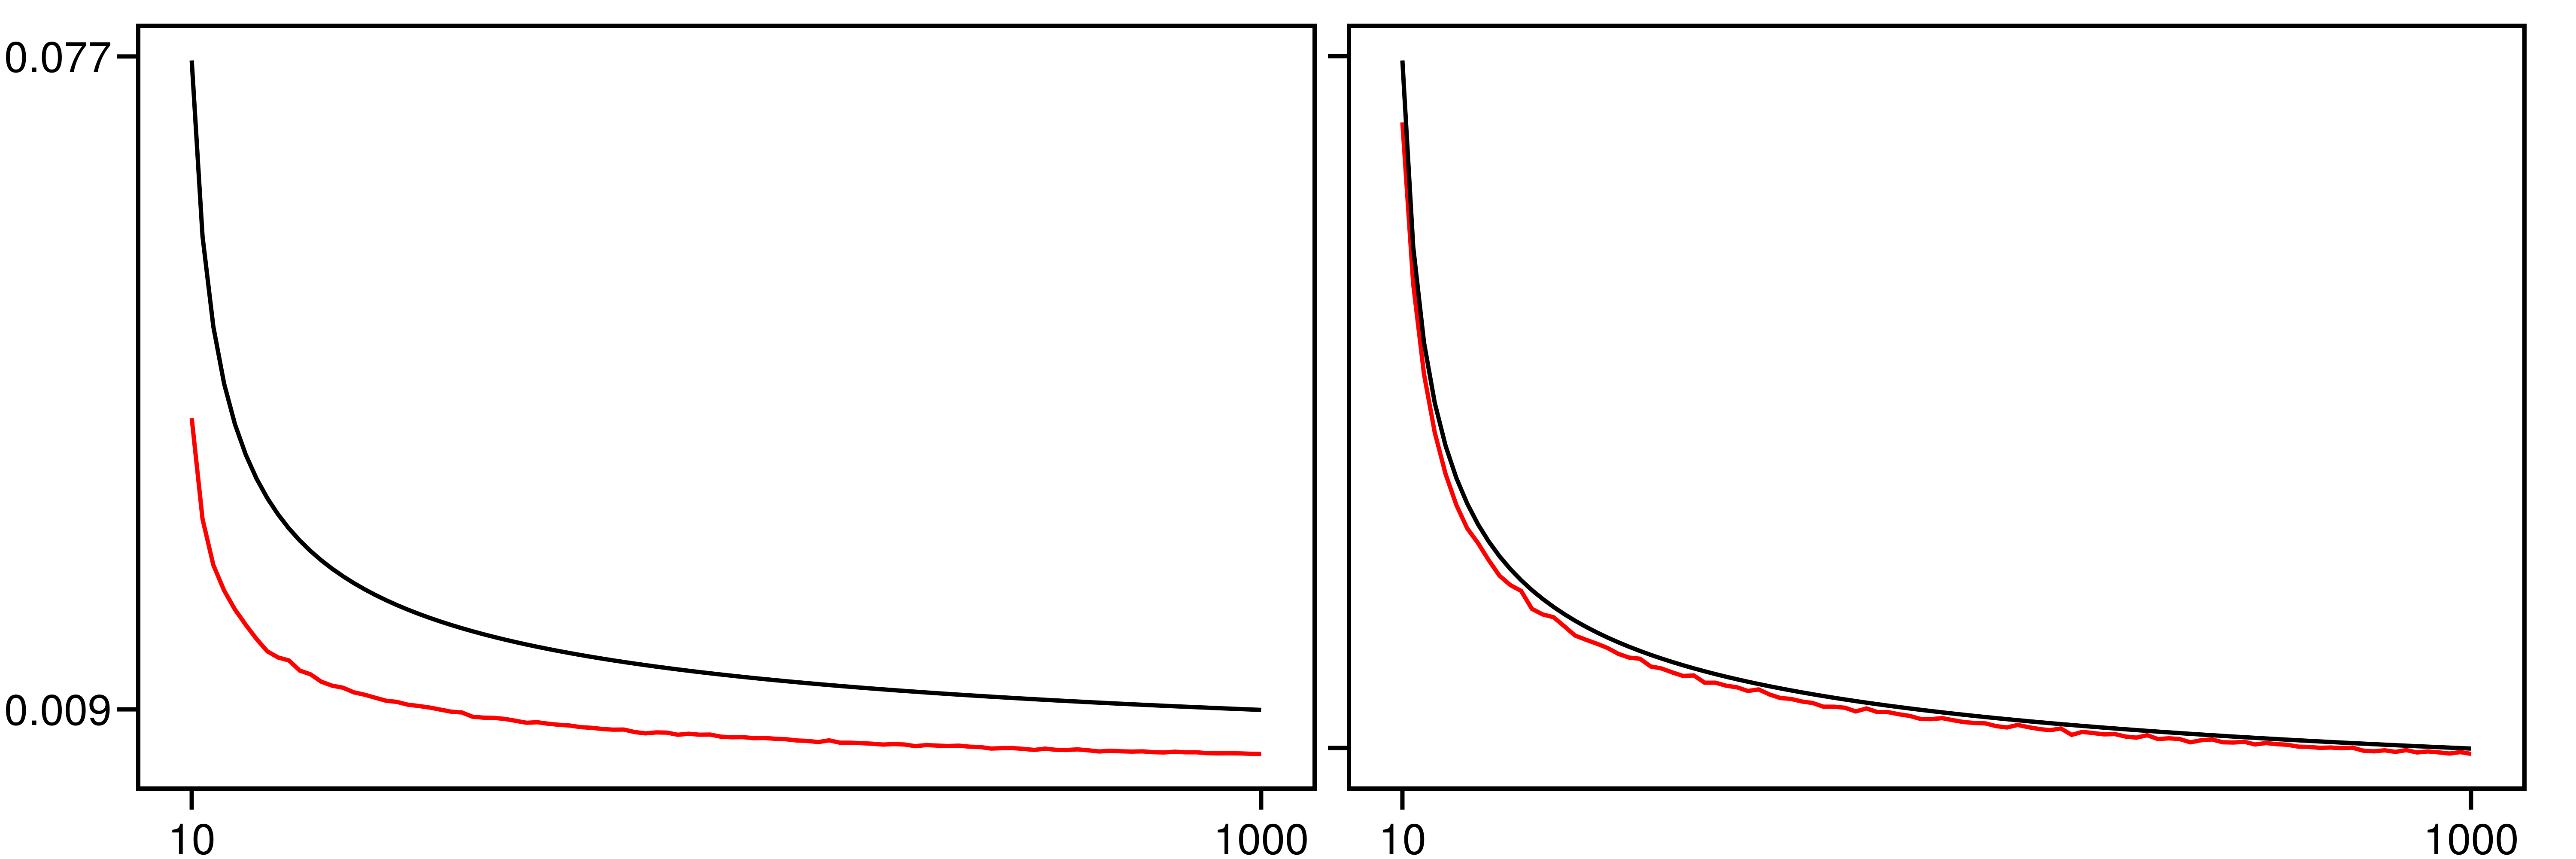
\includegraphics[keepaspectratio, width=\textwidth]{../figures/fig2.5.2.4.png}
    \caption{Comparison between the convergence with $n$ of the expected error (red lines) averaged over an ensemble of $5\cdot10^{3}$ measurements and the square root of the upper estimate \eqref{eq2.5.2.20} (solid black lines) for the same fit of Figure \ref{fig2.5.2.2}.}
    \label{fig2.5.2.4}
\end{figure}
\end{document}
